Knowledge of projective geometry is vital to understanding elliptic curves, as they are curves that are defined in the projective plane.
Therefore from now on, unless otherwise stated, we assume to be working in $\pn[2]$.
As with all projective curves though, it is possible to visualise parts of elliptic curves as they appear in the affine plane.
\begin{definition}
	An \emph{elliptic curve} is a regular, projective cubic curve.
\end{definition}
Here, a cubic simply means that the polynomial that defines the curve is of degree three.
Generally, we use the letter $E$ for an elliptic curve.

So for example, $E(X,Y,Z) = \frac{1}{3}X^3 + 2YZ^2 + 7Y^3$ defines the elliptic curve $E(X,Y,Z) = 0$.
Since $E$ is a homogeneous polynomial of degree three, it suffices to check that there are no singular points.
\begin{align}
	E_X = X^2 \label{deriv-1}\\
	E_Y = 2Z^2 + 21Y^2 \label{deriv-2}\\
	E_Z = 4YZ \label{deriv-3}
\end{align}
Suppose that $E_X = E_Y = E_Z = 0$ at a point $P = [X,Y,Z]$.
\Cref{deriv-1} implies that $X=0$.
\Cref{deriv-3} now implies that either $Y=0$ or $Z=0$.
Either way, \cref{deriv-2} subsequently implies that $X = Y = Z = 0$, which is not a valid point in homogeneous coordinates.
Therefore, there are no singular points on the curve $E$ and it is indeed an elliptic curve.

The following theorem gives a fundamental property of elliptic curves.
\begin{theorem}
	Let $E$ be an elliptic curve.
	Then $E$ has at least one flex in $\pn[2]$.
	\label{flex-existence}
\end{theorem}
\begin{proof}
	We do not prove this theorem, but instead refer readers to \cite[§12]{bix2006} for more information.
\end{proof}
\subsubsection{Bézout's theorem}
Before we go into more detail on elliptic curves, we require an important theorem of Bézout.
\begin{theorem}
	Let $F$ and $G$ be curves in $\pn(k)$ of degree $d_F$ and $d_G$ respectively.
	Suppose that $k$ is algebraically closed, $F$ and $G$ have no common factors and we count each intersection point with its intersection multiplicity.
	Then $F \cap G$ has intersection multiplicity $= d_F d_G$.
	\label{bezouts-theorem}
\end{theorem}
This is \emph{Bézout's theorem}, which is a fundamental result in projective geometry.
Each assumption of Bézout's theorem is important, as each is required for the theorem to hold.
This is one reason why we take the base field $k$ of affine and projective space to be $\C$.
\begin{proof}
	Again, we do not prove Bézout's theorem as it is lengthy and not insightful.
	We refer readers to \cite{silverman2009} or \cite{bix2006}.
\end{proof}
\subsubsection{The addition law on elliptic curves}
Our interest in elliptic curves is mainly due to a special property of theirs.
It is possible to turn the set of points of an elliptic curve $E$ into an abelian group by introducing an addition law that satisfies all of the group axioms.
We do not prove this in this document but direct readers to \cite{silverman2009}.
\begin{figure}[htbp]
	\centering
	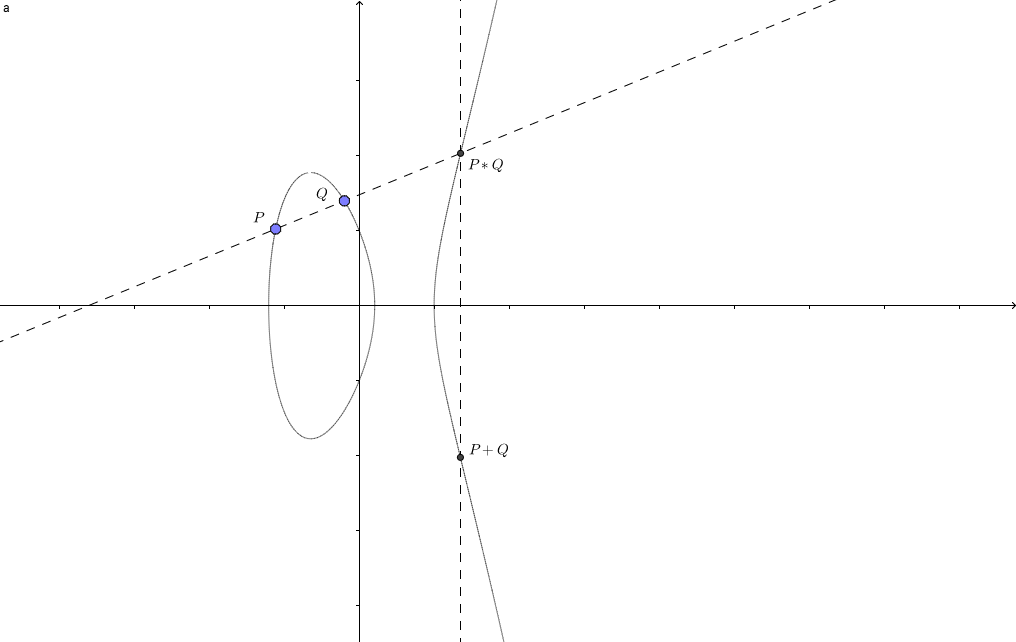
\includegraphics[scale=0.3]{../Figures/ellipticaddition.png}
	\caption{The chord-tangent law $*$ and the addition law $+$ on an elliptic curve}
	\label{ellipticaddition}
\end{figure}
The addition rests upon the so-called `chord-tangent~law', which is illustrated in \cref{ellipticaddition}, along with the full addition operation.
% chord tangent example?
Since an elliptic curve is cubic and regular, every line intersects it with multiplicity exactly three.
This means that given two points (not necessarily distinct), the line on which those points lie (or the tangent line to the curve at the point, if the points are the same) will intersect the curve in exactly one other place.
The chord-tangent law $*$ for two points $P,Q \in E$ is that we define $P * Q$ to be the third point of intersection on the line containing $P$ and $Q$ (which may be $P$ or $Q$ again, if they intersect $E$ with multiplicity greater than 1).

However, the chord-tangent~law alone is not enough to turn $E$ into a group, since the operation is not associative, as is required by a group operation.
This can be remedied, though, by defining the elliptic curve addition law as follows.
\begin{theorem}
	For points $P$, $Q$ and $R$ on an elliptic curve with a flex $\pai$, the addition law $+$ defined by
	$$P + Q = \pai * (P * Q)$$
	turns the curve into an abelian group, where $*$ is the chord-tangent~law.
	The flex $\pai$ acts as the identity element of the group.
\end{theorem}
This is known as Poincaré's theorem.
Note that \cref{flex-existence} ensures that there will be a flex on the curve we can take to be $\pai$.
\begin{proof}
	Let $P,Q,R \in E$.
	We have
	$$P + Q = \pai * (P * Q) = \pai * (Q * P) = Q + P,$$
	so $+$ is commutative.
	Also,
	$$\pai + P = \pai * (\pai * P) = P$$
	because $P$, $\pai$ and $\pai P$ are the three intersection points of the line through $P$ and $\pai$ with $E$.
	Therefore $\pai$ is indeed the identity element, and $-P = \pai * P$.
	Finally, to show associativity,
	\begin{align*}
		P * (Q + R) &= P * (\pai * ( Q * R))\\
		&= ((P*Q)*Q)*(\pai*(QR))\\
		&= ((P*Q)*\pai)*(Q*(Q*R))\\
		&= (\pai * (P*Q))*R\\
		&= (P + Q) * R
	\end{align*}
	and thus $P + (Q + R) = \pai * (P * (Q + R)) = \pai *((P + Q) * R) = (P + Q) + R.$
\end{proof}

Formulas exist which allow this addition to be easily calculated, which we postpone providing until the following section.
\subsubsection{Canonical forms of elliptic curves}
As we have introduced them so far, elliptic curves have no specific form, other than being defined by a homegeneous polynomial of degree three.
The following theorem is useful when working with elliptic curves.
\begin{theorem}
	For any elliptic curve given by a polynomial $E$, there exist projective transformations which put $E$ into one of the following forms:
	\begin{itemize}
		\item $Y^2Z - F(X,Z) = 0$ where $F(X,Z) = X^3 + aX^2Z + bXZ^2 + cZ^3$ for some $a,b,c\in k$
		\item $Y^2Z - F(X,Z) = 0$ where $F(X,Z) = 4X^3 - pXZ^2 - qZ^3$ for some $p,q\in k$
	\end{itemize}
	In either form, the curve is regular if and only if $f(x)$, the dehomogenisation of $F(X,Z)$, has no repeated roots.
	The point $\pai = [0,1,0]$ is the unique point at infinity on the curve, and is a flex.
	The line at infinity $Z = 0$ is tangent to $E$ at $\pai$.
\end{theorem}
When dehomogenising these forms, notice that we have the affine curves $y^2 = x^3 + ax^2z + bxz^2 + cz^3$ and $y^2 = 4x^3 - pxz^2 - qz^3$.
Since $\pai = [0,1,0]$ acts as the identity on curves of this form, the elliptic curve addition law is sometimes stated as $P + Q$ equals the reflection of $P * Q$ in the $x$-axis, as in \cref{ellipticaddition}.

When a curve is in the first form given, we say that it is in \emph{normal form}.
When in the second form, we say that it is in \emph{Weierstrass form}.
\begin{proof}
	Again, we do not prove this theorem due to its length, but refer readers to \cite{323-lectures,bix2006}.
\end{proof}
